\begin{savequote}[75mm]
I've often said that my rats have taught me much more than I've taught them.
\qauthor{B. F. Skinner}
\end{savequote}

\chapter{Experiment description}
\label{chap:experiment}

\section{The task}
    The subjects were 8 adult naive male Wistar rats (12 - 16 weeks old, 380 - 400g). The animals were housed individually in a 12h light/dark cycle with the light turned on at 7am. They were food-deprived to gradually reach and then maintain 85\% of their free-feeding weight. Animals were handled according to the experimental protocol approved by UFABC's Ethics Committee (Comitê de Ética de Uso Animal CEUA-UFABC). All procedures were conducted during the light cycle.
    
    Animals were trained in an operant chamber developed in our laboratory, totally controlled by an Arduino uno, and made of acrylic plastic. The box has a \textit{nosepoke}, which is a hole equipped with an infrared emitter-sensor that detects when the animal inserts its snout. In the same wall there is a drinker coupled to a lickometer, which is a nozzle that the animal licks to obtain water-sucrose solution. Before the nozzle there is a gate, controlled by an arduino board coupled to a stepper motor, that limits the animal access. 
    
    \begin{figure}
        \centering
        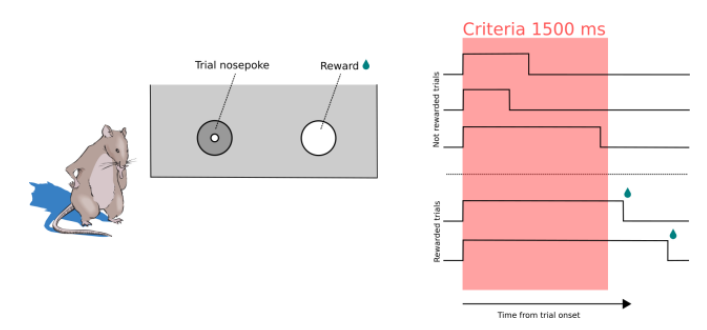
\includegraphics[width=\textwidth]{figures/tarefa_eli.png}
        \caption[Our DRRD task]{Our DRRD task. If the animal stays in the nosepoke for longer than the criteria, it can collect a reward. Taken with permission from \cite{Eliezyer2018}}
        \label{fig:task}
    \end{figure}

\section{Training schedule}
    First, the animals were trained to nose poke in a continuous schedule of reinforcement (CR), in which every nosepoke was rewarded independent of duration. To conclude this phase the animal had to nose poke at least 100 times on a 60 minutes session. Animals had at most one training session per day, both in CR and in the subsequent DRRD. 
    
    After reaching this performance,the animals were trained with a Differential Reinforcement of Response Duration (DRRD) procedure: Only long trials were rewarded. In order to receive the reward (four licks of a 50\% glucose solution), the animal had to poke the hole and hold for a time equal or longer than the defined criterion of 1500ms. The trials were self initiated and self ended, and even when the animal didn't reached the time criteria it was free to start a new trial. All sessions were video recorded.

\section{Rationale}
    The central distinction of this version of the DRRD task is the speed of behavior acquisition. It was developed by our group to enable recording of neurons through learning in a single session, and most of the specifics of this task were defined with this aim.
    
    Previous DRRD protocols have a window of reinforcement with criteria for minimum and maximum time, thus if the animal holds nosepoking for too long it receives no reward. We removed this second criterion to speed up training \cite{}, and justify that the challenge the subjects engage with is still one of timing -- as opposed to impulse control and waiting for as long as possible. We argue that the incentive to get reward as soon as possible is an intrinsic one or occurs naturally, and thus we don't need to enforce a penalty for longer responses. In fact, behavioral results indicate this is the case: animals' responses peak around the criterion, and very long responses are uncommon.